%----------------------------------------------------------------------
% Poster for MathPsych/Psychonomics 2017
% ---------------------------------------------------------------------

\documentclass[paperheight=36in,paperwidth=48in,landscape]{baposter}
\usepackage{amsmath}
\usepackage{relsize}  % For \smaller
\usepackage{url}      % For \url
\usepackage{tikz}
\usetikzlibrary{bayesnet}
\usetikzlibrary{arrows}


\usepackage{sansmathfonts}
\usepackage[T1]{fontenc}
\renewcommand*\familydefault{\sfdefault}

%%% Global Settings %%%%%%%%%%%%%%%%%%%%%%%%%%%%%%%%%%%%%%%%%%%%%%%%%%%%

\graphicspath{{figures/}}  % Root directory of the pictures 
% \tracingstats=2  % Enabled LaTeX logging with conditionals

%%% Color Definitions %%%%%%%%%%%%%%%%%%%%%%%%%%%%%%%%%%%%%%%%%%%%%%%%%%

\definecolor{bordercol}{RGB}{40,40,40}
\definecolor{tarletonPurple}{RGB}{79,45,127}
\definecolor{headerfontcol}{RGB}{0,0,0}
\definecolor{boxcolor}{RGB}{255,255,255}
\definecolor{backgroundcolor}{RGB}{229,224,236}

%%%%%%%%%%%%%%%%%%%%%%%%%%%%%%%%%%%%%%%%%%%%%%%%%%%%%%%%%%%%%%%%%%%%%%%%
%%% Utility functions %%%%%%%%%%%%%%%%%%%%%%%%%%%%%%%%%%%%%%%%%%%%%%%%%%

%%% Save space in lists. Use this after the opening of the list
\newcommand{\compresslist}{
	\setlength{\itemsep}{1pt}
	\setlength{\parskip}{0pt}
	\setlength{\parsep}{0pt}
}

%%%%%%%%%%%%%%%%%%%%%%%%%%%%%%%%%%%%%%%%%%%%%%%%%%%%%%%%%%%%%%%%%%%%%%%%%
%%% Document Start %%%%%%%%%%%%%%%%%%%%%%%%%%%%%%%%%%%%%%%%%%%%%%%%%%%%%%
%%%%%%%%%%%%%%%%%%%%%%%%%%%%%%%%%%%%%%%%%%%%%%%%%%%%%%%%%%%%%%%%%%%%%%%%%

\begin{document}
\typeout{Poster rendering started}

%%% General Poster Settings %%%%%%%%%%%%%%%%%%%%%%%%%%%%%%%%%%%%%%%%%%%%
%%%%%% Eye Catcher, Title, Authors and University Images %%%%%%%%%%%%%%%
\begin{poster}{
	grid=false,
        columns=6,
    	eyecatcher=true, 
	borderColor=bordercol,
	headerColorOne=tarletonPurple,
        headershade=plain,
	headerFontColor=boxcolor,
	% Only simple background color used, no shading, so boxColorTwo
        % isn't necessary
	boxColorOne=boxcolor,
	headershape=smallrounded,
	headerfont=\Large\sf\bf,
	textborder=roundedsmall,
	background=plain,
        bgColorOne=backgroundcolor,
        bgColorTwo=yellow,
        headerborder=open,
        boxshade=plain
}
%%% Eye Catcher %%%%%%%%%%%%%%%%%%%%%%%%%%%%%%%%%%%%%%%%%%%%%%%%%%%%%%%%%
{
	
\includegraphics[height=0.9\headerheight]{figures/systemSeal.png}
}
%%% Title %%%%%%%%%%%%%%%%%%%%%%%%%%%%%%%%%%%%%%%%%%%%%%%%%%%%%%%%%%%%%%%
{\huge\bf
  A hierarchical Bayesian model for measuring response times in a mental arithmetic task
}
%%% Authors %%%%%%%%%%%%%%%%%%%%%%%%%%%%%%%%%%%%%%%%%%%%%%%%%%%%%%%%%%%%
{
  {Thomas J. Faulkenberry}\\
  { Department of Psychological Sciences, Tarleton State University}\\
}
%%% Logo %%%%%%%%%%%%%%%%%%%%%%%%%%%%%%%%%%%%%%%%%%%%%%%%%%%%%%%%%%%%%%%
{
  
\includegraphics[height=0.9\headerheight]{figures/tarletonLogo.jpg}
}

\headerbox{Response time distributions}{name=rts,span=2,column=0,row=0}{
  Response times (RTs) have long been one of the primary measures of cognitive processing, especially in mental arithmetic \cite{ashcraft}. The classic method for analyzing RTs consists of collapsing the (often positively skewed) distribution of RTs to a single number (e.g., mean or median). 

\begin{minipage}{0.6\textwidth}
  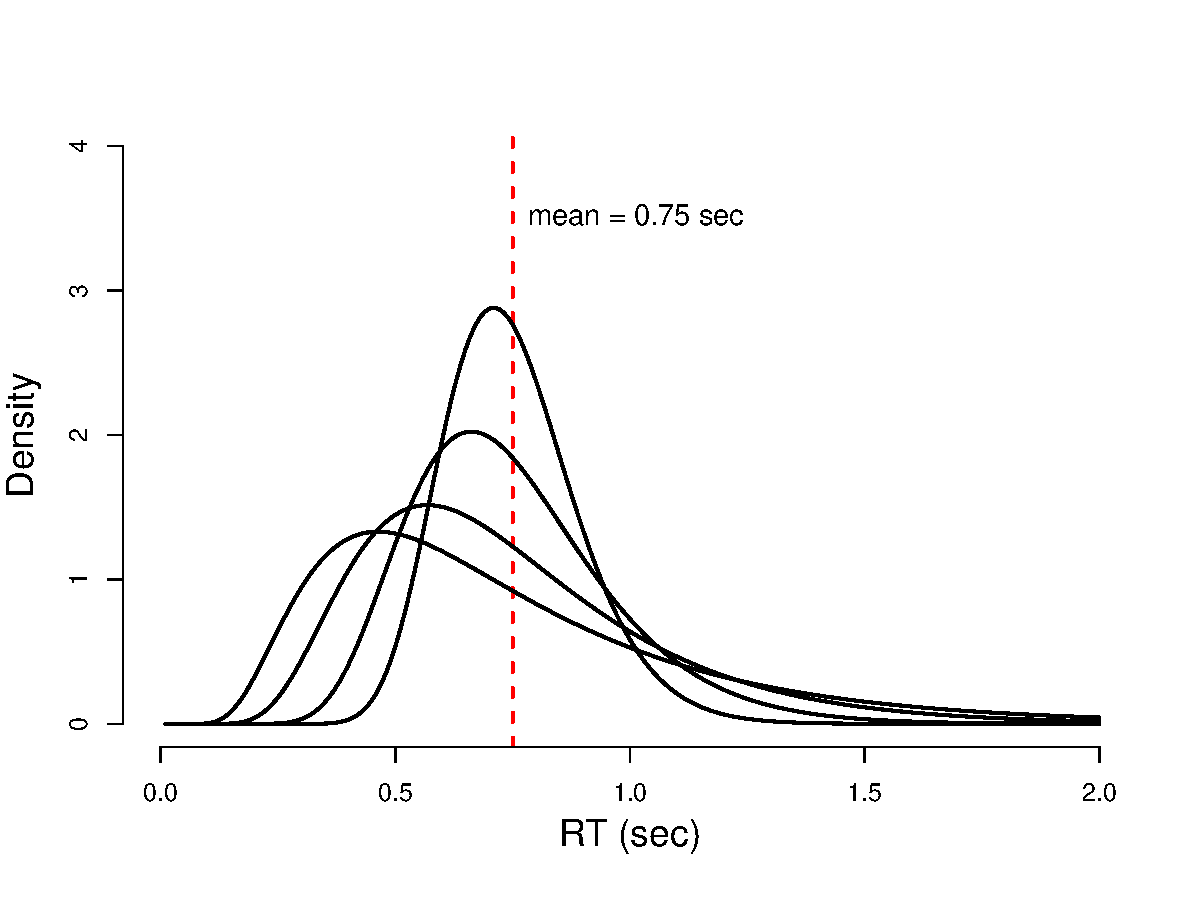
\includegraphics[width=\linewidth]{figures/rtPlots.pdf}
\end{minipage}%
\begin{minipage}{0.4\textwidth}
However, this method can result in a loss of measurement resolution, particularly for skewed distributions. Notice how RT distributions of multiple scales/shapes can collapse to the same mean. Thus, by focusing solely on the center, we lose much information about the scale and shape of the distribution.
\end{minipage}

The purpose of the present study was to develop a hierarchical Bayesian model for estimating the location/scale/shape characteristics of RT distributions in mental arithmetic.
}

\headerbox{The shifted Wald distribution}{name=wald, span=2, column=0, below=rts}{

  The current model is based on a shifted Wald distribution \cite{anders,faulkenberry2017,matzke}, which represents the density of first-passage times for a single-boundary diffusion process. As a descriptive model for RTs, it provides a three-parameter location/scale/shape characterization.  The probability density is given by:

  \[
f(x) = \frac{\alpha}{\sqrt{2\pi(x-\psi)^3}}\exp \Biggl(-\frac{(\alpha - \gamma(x-\psi)^2)}{2(x-\psi)}\Biggr)
\] 

\vspace{2mm}

The effects of varying each parameter can be seen below:

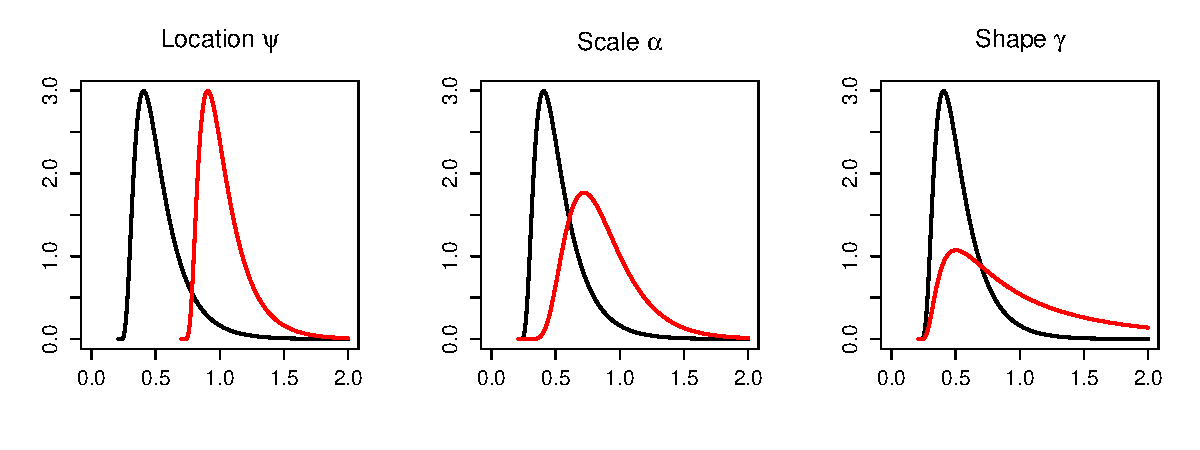
\includegraphics[width=\linewidth]{figures/waldParams.pdf}

}

\headerbox{Data}{name=data, span=2, column=0, below=wald, above=bottom}{
  I measured trial-by-trial RTs for 20 undergraduates who completed an addition verification task. On each trial, participants were asked to quickly indicate whether problems were True or False via a button press.

\begin{minipage}{0.5\textwidth}
  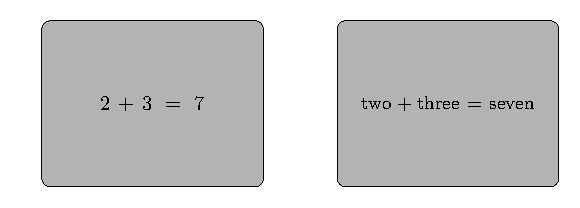
\includegraphics[width=\linewidth]{figures/experiment.pdf}
\end{minipage}%
\begin{minipage}{0.5\textwidth}
  Across 288 trials, I manipulated \\
  problem size (small, large), \\
  problem format (digits, words),\\
  and truth value (true, false).
    \end{minipage}
  }

\headerbox{Hierarchical Bayesian model}{name=model, span=2, column=2,row=0}{

  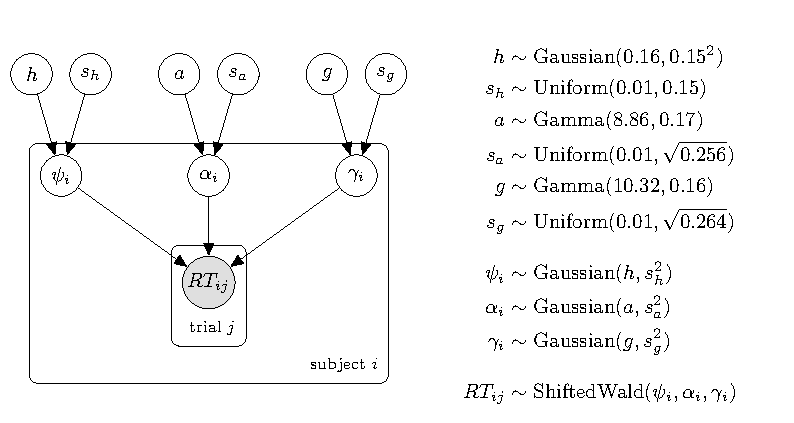
\includegraphics[width=\linewidth]{figures/bayesModel.pdf}

  RTs are assumed to be drawn from a shifted Wald distribution, where parameters $\psi_i$ (location), $\alpha_i$ (scale), and $\gamma_i$ (shape) are assumed to vary by participant.  In turn, the individual location/scale/shape parameters are assumed to be drawn from group-level distributions. The group-level priors are based on previous model fits obtained in \cite{faulkenberry2017}. 
}

\headerbox{Posterior distributions of location/scale/shape}{name=posterior, span=2, column=2, below=model, above=bottom}{
  Posterior distributions for the group-level parameters were separately estimated for each experimental condition defined by crossing the factors of problem size, format, and truth value:\\

  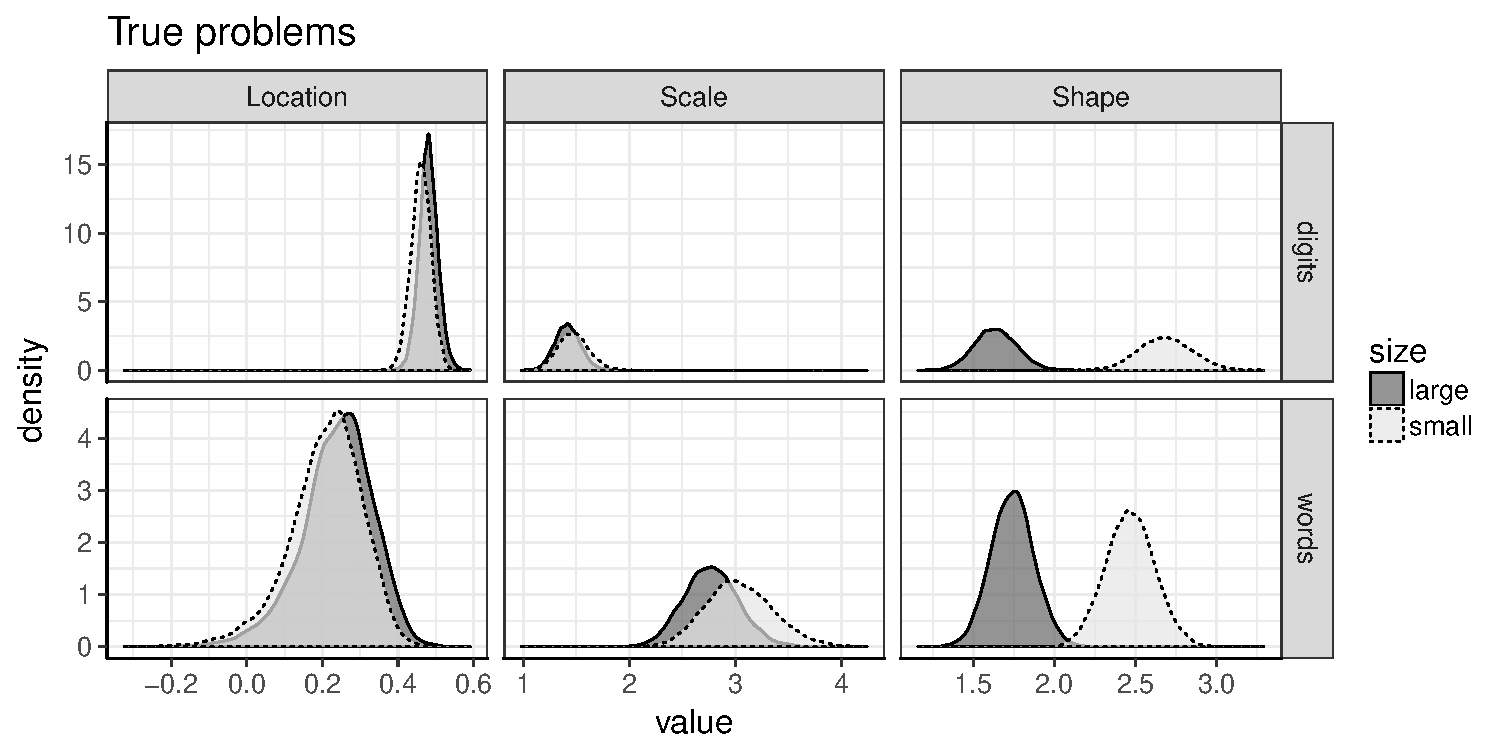
\includegraphics[width=\textwidth]{figures/posteriorTrue.pdf}


  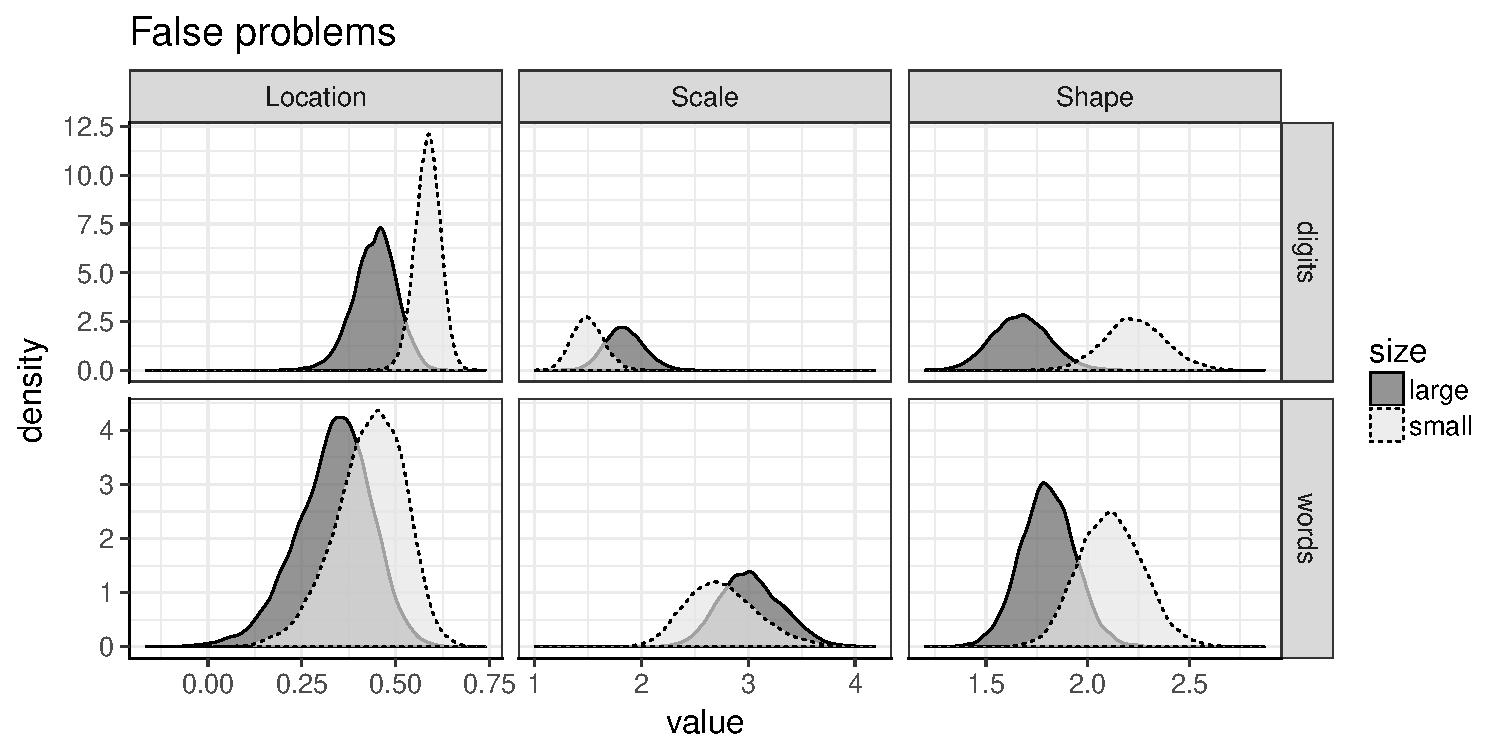
\includegraphics[width=\textwidth]{figures/posteriorFalse.pdf}
}

\headerbox{Posterior predictive checks}{name=predictive, span=2, column=4,row=0}{

  I performed a posterior predictive check for each of the model fits. For each experimental condition, I randomly chose 20 samples from the posterior chains for each of the location, scale, and shape parameters.  Then, I generated the corresponding shifted Wald densities corresponding to each random sample. Below are the histograms of actual RTs along with the simulated shifted Wald densities for True problems (False problems presented a similar picture).  The similarities between the data (histogram) and the simulated data (densities) show that the model fits were adequate.

  \begin{minipage}{0.5\textwidth}
    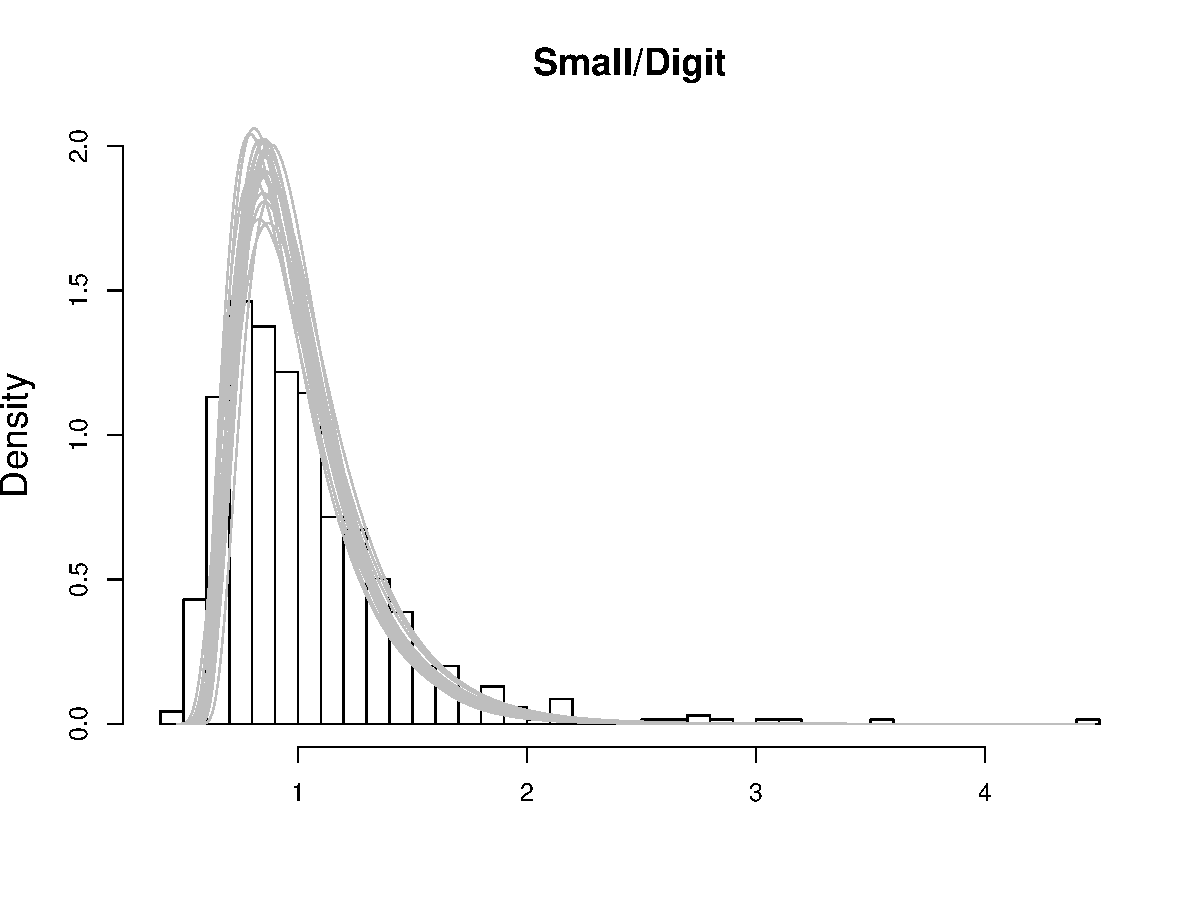
\includegraphics[width=\linewidth]{figures/pred-smallDigit.pdf}
  \end{minipage}%
  \begin{minipage}{0.5\textwidth}
    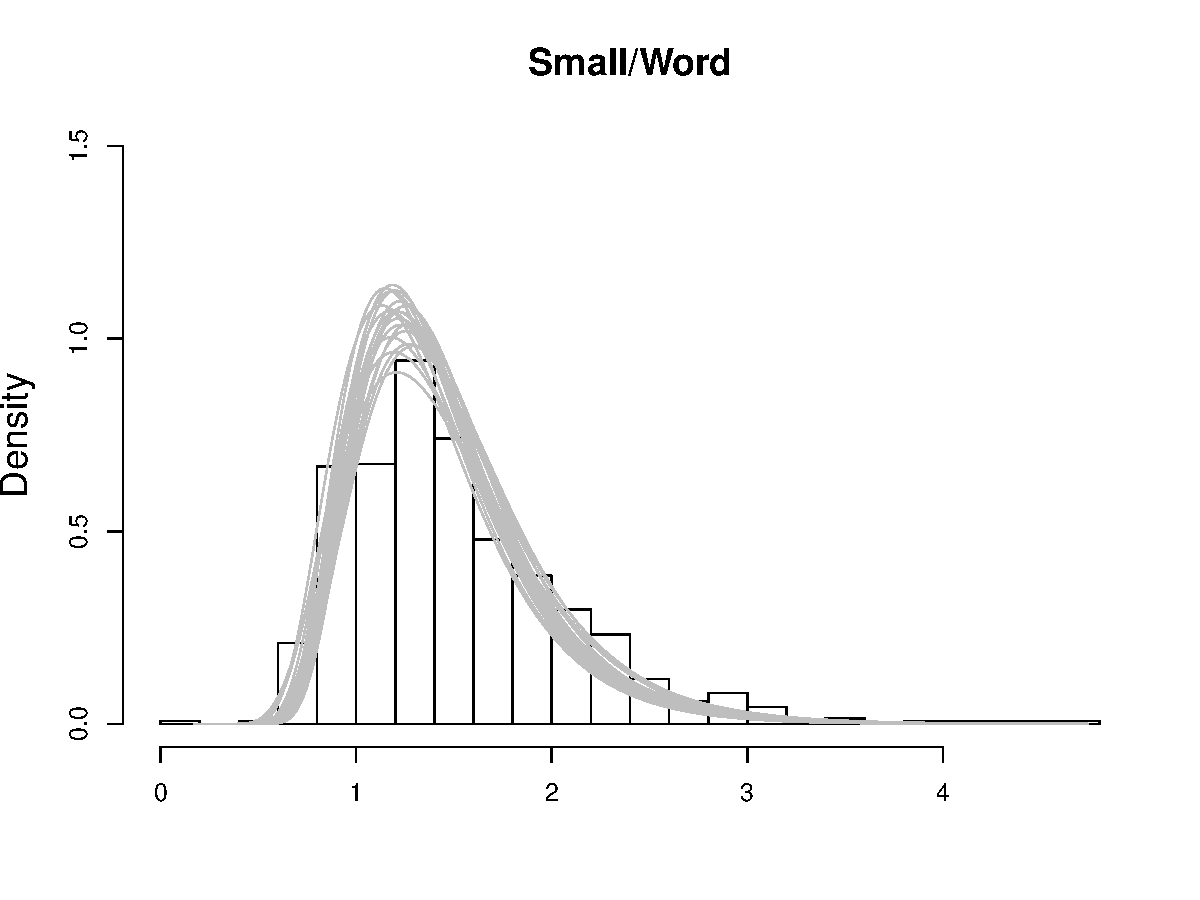
\includegraphics[width=\linewidth]{figures/pred-smallWord.pdf}
  \end{minipage}

  \begin{minipage}{0.5\textwidth}
    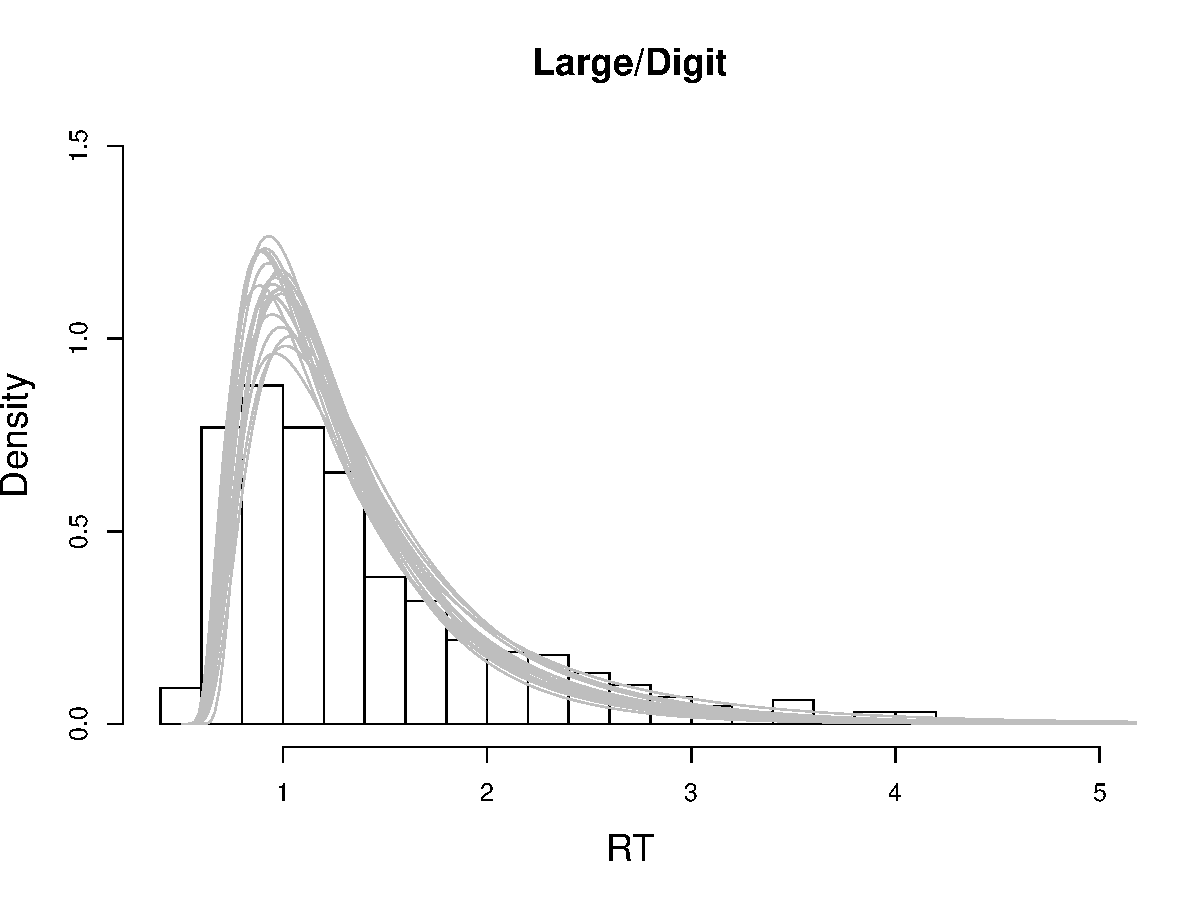
\includegraphics[width=\linewidth]{figures/pred-largeDigit.pdf}
  \end{minipage}%
  \begin{minipage}{0.5\textwidth}
    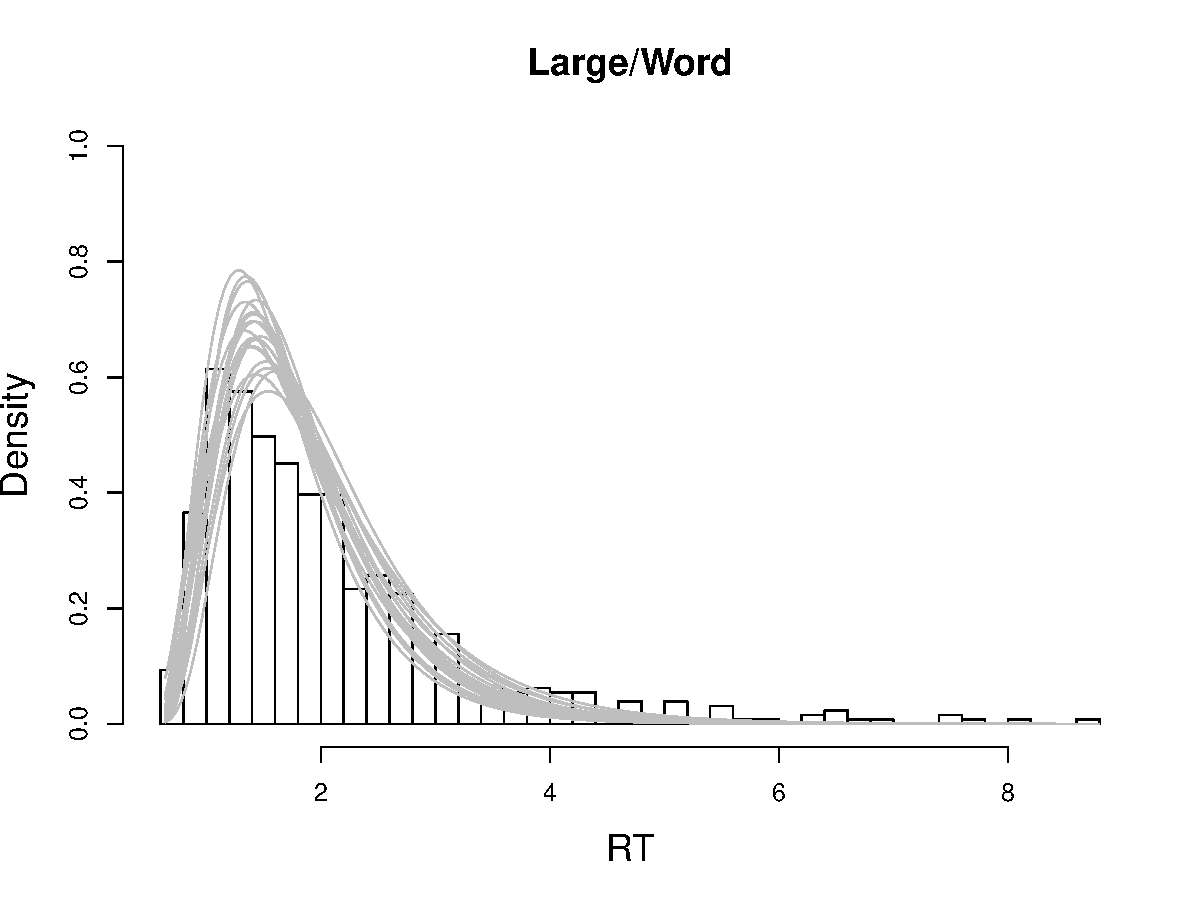
\includegraphics[width=\linewidth]{figures/pred-largeWord.pdf}
  \end{minipage}
 
}

\headerbox{Conclusions and speculations}{name=conclusion, span=2,column=4,below=predictive}{
  The hierarchical Bayesian model presented here has the potential to be informative for modeling response times in mental arithmetic. For example, some initial observations are:

  \begin{enumerate}
  \item Manipulating problem format affects {\bf location and scale}, but not {\bf shape}, possibly reflecting cognitive processes related to response caution and encoding/production.
    \item Manipulating problem size primarily affects {\bf shape}, indicating that large problems may be solved using fundamentally different types of processing compared to small problems.
    \end{enumerate}


}

\headerbox{References}{name=references,span=2,column=4,below=conclusion,above=bottom}{
\small % Make the whole text smaller
%\vspace{-0.5em} % Save some space at the beginning
\bibliographystyle{plain} % Use plain style
\renewcommand{\section}[2]{\vskip 0.05em} % Omit "References" title
\begin{thebibliography}{1} % Simple bibliography with widest label of 1
\itemsep=-0.05em % Save space between the separation
\setlength{\baselineskip}{0.4em} % Save space with longer lines

\bibitem{anders} Anders, R., Alario, F., \& Van Maanen, L. (2016). The shifted Wald distribution for response time data analysis. {\it Psychological Methods, 21}(3), 309-327.

\bibitem{ashcraft} Ashcraft, M. H. (1992). Cognitive arithmetic: A review of data and theory. {\it Cognition, 44}(1-2), 75-106.
  
\bibitem{faulkenberry2017} Faulkenberry, T. J. (2017). A single-boundary accumulator model of response times in an addition verification task. {\it Frontiers in Psychology, 8}:1225.

\bibitem{matzke} Matzke, D., \& Wagenmakers, E.-J. (2009). Psychological interpretation of the ex-Gaussian and shifted Wald parameters: A diffusion model analysis. {\it Psychonomic Bulletin \& Review, 16}(5), 798-817.  
\end{thebibliography}
}

\end{poster}
\end{document}
